\documentclass[tikz]{standalone}
\usepackage{amsmath,amssymb,multirow}
\usetikzlibrary{shapes.misc, positioning,automata,arrows,calc,fit}
\tikzset{VertexStyle/.style = {draw,circle,thick,
		minimum size=1cm,
		font=\Large\bfseries},thick} 
\begin{document}
  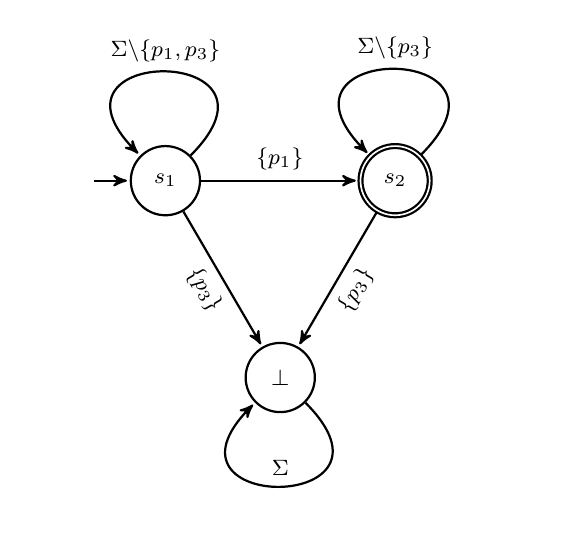
\begin{tikzpicture}[->,>=stealth',shorten >=1pt,thick,initial text=$ $,align=center,node distance=5mm,font=\footnotesize]
\thickmuskip=0mu
\node[state,initial] (SA)  {$s_1$};
\path (SA) edge[loop] node[midway,above] (W1) {$\Sigma\backslash\{p_1,p_3\}$} (SA);
\node[state,accepting,right =2cm of SA] (ST) {$s_2$};
\path (ST) edge[loop] node[midway,above] (W2) {$\Sigma\backslash\{p_3\}$} (ST);
\draw[->] (SA) -- (ST) node[midway,above] {$\{p_1\}$};
\node[state] (bot) at ($(SA)!0.5!(ST)-(0,2.5)$) {$\bot$};
\draw[->] (SA) -- (bot) node[midway,below,sloped] {$\{p_3\} $} ;
\draw[->] (ST) -- (bot) node[midway,below,sloped] {$\{p_3 \}$} ;
\draw (bot) to [in=225,out=315,looseness=8] node[midway,above] (W3) {$\Sigma$} (bot);
  \end{tikzpicture}
\end{document}